% LTeX: language=de-DE
\chapter{Konzeption}
	%
	Um Konsistenz mit Literatur und Marktrecherchen sicherzustellen werden im Rahmen dieser Arbeit technische Begriffe aus der Skaterszene genutzt.
	Während \textit{Skateboarding} einerseits keinesfalls als neuartiges Phänomen zu bezeichnen ist und  andererseits in den vergangenen fünf Jahren eine Renaissance erlebt hat, kann nicht davon ausgegangen werden, dass alle Lesenden mit der Terminologie vertraut sind.
	Daher wird im Folgenden zunächst Fokus auf eine Begriffskonvention gelegt und in diesem Rahmen funktionale Kernkomponenten eines Skate- bzw. Longboards\footnote{Baulich zwar leicht zu unterscheiden, jedoch aus den gleichen Kernkomponenten und -funktionalitäten aufgebaut.}~erläutert.\par\medskip
	%
	Das Antriebssystem soll in ein bestehendes, übergeordnetes System bestehend aus mechanischen und elektronischen Komponenten eingebettet werden.
	Sowohl das übergeordnete System, als auch die Einsatzumgebung definieren konstruktive Einschränkungen, die in einem weiteren Unterkapitel herausgearbeitet werden sollen.\par\medskip
	%
	Zuletzt sollen vor dem Hintergrund der zuvor festgelegten Rahmenbedingungen Designziele definiert und erste Designideen konkretisiert werden.
	Unterstützt wird dies durch Markt- und Literaturrecherche.
	%
	\section{Funktionale Komponenten eines Longboards}
		%
		Historisch ergaben sich esoterische Namenskonventionen für Teilkomponenten von Skate- und Longboards.
		Während sie im einfachsten Fall unabhängig vom jeweiligen Sprachraum mit ihren jeweiligen englischen Begriffen zu finden sind, weichen Bezeichnungen Teilweise aber auch stark von in der Industrie verbreiteten Bezeichnungen ab.
		Um dieser Konvention zu folgen, sollen hier zunächst die Teilkomponenten kurz beschrieben werden.\par\medskip
		%
		\begin{figure}[h]
			\centering
			\includesvg[width=.9\textwidth]{Footage/AwesomeBoard Transmission CAD/Drawings/Longboard.svg}
			\caption[Grundlegender Aufbau eines Longboards]{Grundlegender Aufbau eines Longboards. 15~Deck, 16~Truck Bolts, 17~Truck Bolt Nuts, 18~Riser Pad.}\label{fig:longboard}
		\end{figure}
		%
		\Cref{fig:longboard} zeigt zunächst den grundlegenden Aufbau eines Longboards.
		Erkennbar sind hier vordergründig das Deck~(15), welches die fahrende Person trägt und hierbei einen Großteil der wirkenden Kräfte aufnehmen muss.
		Je nach Fahrstil werden weichere oder härtere Materialien gewünscht um etwa Unebenheiten des Untergrundes auszugleichen oder die Ausführung von Tricks\footnote{Über die rein laterale Fortbewegung hinausgehende, meist kunstvoll ausgeführte Bewegungen des Boards mit und unter den Füßen.}~positiv zu beeinflussen.\linebreak
		Meist kommt hier Schichtholz mit oder ohne eingearbeitetem Glas-, Aramid- oder Kohlefasergewebe zum Einsatz, es sind bisweilen aber auch exotischere Materialien wie Aluminium, ABS\footnote{Acrylnitrilbutadienstyrol.}~vertreten.\nomenclature[A]{ABS}{Acrylnitrilbutadienstyrol}
		In \cref{fig:longboard} befinden sich links und rechts, zentral entlang der Längsachse des Decks angeordnet die Trucks genannten Baugruppen zusammen mit jeweils zwei Rollen.
		Eine mechanisch belastbare Verbindung zum Deck wird durch \textit{Truck Bolts}~(16) und \textit{Truck Bolt Nuts}~(17) hergestellt.
		Im Longboarding üblicher, als bei den mit deutlich kleineren Rollen ausgestatteten Skateboards werden zwischen Deck und Truck häufig \textit{Riser Pads}~(18) eingesetzt.
		Hier handelt es sich um aus flexiblem Material verschiedener Härtegrade gefertigte Pufferplatten mit Doppelfunktion.
		Einerseits unterstützen sie die Entkopplung der Füße von Vibration und verhindern sogenannte \textit{Wheel Bites} -- ein Kontakt des Decks mit den Rollen während eines Lenkmanövers mit meist fataler Konsequenz.\par
		%
		\begin{figure}[h]
			\centering
			\includesvg[height=.6\textheight]{Footage/AwesomeBoard Transmission CAD/Drawings/Drivetrain - Truck}
			\caption[Explosionsansicht eines der Trucks]{Aufbau eines der Trucks als Explosionsansicht exemplarisch an einem \textsc{Caliper II}. Sichtbar sind hier: 1~Baseplate, 2~Pivot Cup, 3~Kingpin, 4~Hanger, 5~RS Bushing, 6~BS Bushing, 7~BS Washer, 8~RS Washer, 9~Kingpin Nut.}\label{fig:caliper exploded}
		\end{figure}
		%
		Der Aufbau der Trucks selbst wird in \cref{fig:caliper exploded} exemplarisch am Typ \textsc{Caliber II} gezeigt.
		Der \textit{Hanger}~(4) bildet hier das zentrale Bauteil und muss den Großteil der wirkenden Kräfte aufnehmen.
		Er wird drehbar in der \textit{Baseplate}~(1) gleitend gelagert.
		Würden der \textit{Hanger} und die \textit{Baseplate} in direkten Kontakt kommen, so käme es zu erhöhtem Abrieb und reduziertem Gleitverhalten.
		Hier wird ein meist aus POM\footnote{Polyoxymethylen.}~gefertigter \textit{Pivot Cup}~(2) eingesetzt.
		In Position gehalten wird der \textit{Hanger} mittels des \textit{King Pins}~(3) und der \textit{Kingpin Nut}~(9).
		Das Rückstellmoment nach Ende eines Lenkmanövers wird durch zwei vergleichsweise dicke Gummiringe -- \textit{Bushings} genannt -- erzeugt, die mit der \textit{Kingpin}-Achse koaxial beidseitig mit dem Hanger in mechanischem Kontakt stehen.
		Deckseitig befindet sich der \textit{BS Bushing}~(6), straßenseitig angeordnet der \textit{RS Bushing}.\nomenclature[A]{BS}{Board Side}\nomenclature[A]{RS}{Road Side}
		Die Präfixe stehen für Boardside bzw. Roadside und spiegeln ihre Positionen wider.
		Unterschieden wird hier, da sich verschiedene Geometrien und Härtegrade der \textit{Bushings} nicht unabhängig ihrer Position merklich auf das Fahrgefühl und Lenkvermögen auswirken können\footnote{Durch Drehen der \textit{Kingpin Nut} und damit einer Änderung der Vorspannung der \textit{Bushings}~kann hier auch im Feld relativ unkompliziert nachjustiert werden}.
		Um die Lasten besser auf die Oberfläche der \textit{Bushings} zu verteilen werden üblicherweise tellerförmige Scheiben, die \textit{RS} und \textit{BS Washer}~(5,6) auf den \textit{Hanger} abgewandten Seite platziert.\par\medskip
		%
		\begin{figure}[h]
			\centering
			\includesvg[width=.9\textwidth]{Footage/AwesomeBoard Transmission CAD/Drawings/Drivetrain - Wheels NT}
			\caption[Montage der Rollen an der Achse des Hanger]{Montage der Rollen an der Achse des Hangers. Links in explodierter und rechts in Schnittansicht. Zu sehen sind: 10~Rolle, 11~Kugellager, 12~Speedring, 13~Spacer, 14~Achsmutter.}\label{fig:wheel NT exploded}
		\end{figure}
		%
		Je nach gewünschter Laufruhe und in Abwägung zwischen Traktion und Rollwiderstand werden Rollen verschiedener Größen und Materialien drehbar auf den \textit{Hanger}-Achsen gelagert.
		Mit Blick auf \cref{fig:wheel NT exploded} wird Konzentrisch in den Kern der Rolle~(10) -- vergleichbar mit einer Felge, die das weichere Mantelmaterial trägt -- beidseitig jeweils ein 608 Kugellager~(11) platziert.
		Diese Kugellager sind Radialrillenkugellager und gebaut, um besonders gut radiale Kräfte aufnehmen und ableiten zu können.
		Um potenziell destruktive axiale Kräfte in Kurven oder durch das Anzugsmoment der Achsmutter~(14) zu minimieren, wird, ebenfalls in den Kern der Rolle und zwischen die beiden Lager, der \textit{Spacer}~(13) angeordnet.
		Er besteht aus hartem Metall, hat einen Innendurchmesser gleich des nominellen Durchmessers der \textit{Hanger}-Achse, eine Wandstärke von \(\sim \qty{1}{\milli\metre}\) und eine Länge, die gerade so gewählt ist, dass er an beiden Flanken mit den Innenringen der Lager in Kontakt steht, wenn sie beide vollständig im Kern eingelassen sind.
		Ein schleiffreies Laufen der Lager wird durch \textit{Speedrings}~(12) sichergestellt.
		Ihre Dimensionen entsprechen denen des \textit{Spacers}, allerdings mit nur \qty{1}{\milli\metre} eine deutlich geringere Länge.
		Letztlich wird alles mit einer \textit{Achsmutter} auf der \textit{Hanger}-Achse fixiert.
		%
	\section{Konstruktive Rahmenbedingungen}\label{sec:constructive limitations}
		%
		Das Antriebssystem soll in ein bestehendes System aus Batterie, Batteriemanagement, Motorcontrollern und Deck integriert und die Einsatzbedingungen müssen berücksichtigt werden.
		Hieraus ergeben sich konstruktive Rahmenbedingungen, die bei der Planung berücksichtigt werden müssen.
		%
		\subsection{Bestehendes System}
			%
			Die Batterie besteht aus 40~Lithium-Ionen Zellen in 10S4P-Konfiguration vom Typ \textsc{Samsung INR18650-30Q} mit einer nominellen Zellspannung von \qty{3,6}{\volt}, einer Mindestzellentladekapazität von \qty{2950}{\milli\amperehour} und einem maximalen Entladestrom von \qty{15}{\ampere} (vgl.~\cref{tab:cellspecifications} und~\cite{INR18650.30Q.Specs.202202}).
			%
			\begin{table}[h]
				\caption[Zellspezifikationen \textsc{Samsung INR18650-30Q}]{Zellspezifikationen \textsc{Samsung INR18650-30Q}~\cite{INR18650.30Q.Specs.202202}.}\label{tab:cellspecifications}
				\centering
				\begin{tabular}{@{}ll@{}}
					\toprule
					Charakteristik				& Spezifikationen \\ \midrule
					Minimale Entladekapazität	& \qty{2950}{\milli\amperehour} \\
					Nominelle Zellspannung		& \qty{3,6}{\volt} \\
					Standard Ladebedingungen	& CC/CV, \qty{1,5}{\ampere}, \qty{4,2 +- 0,05}{\volt} \\
					Maximale Ladebedingungen	& CC/CV, \qty{4}{\ampere}, \qty{4,2 +- 0,05}{\volt} \\
					Maximaler Dauerentladestrom & \qty{15}{\ampere} bei \qty{25}{\degreeCelsius} \\
					Minimale Zellspannung		& \qty{2,5}{\volt} \\
					Gewicht						& \qty{48}{\gram} \\
					Betriebstemperatur			& Laden: \qtyrange{0}{50}{\degreeCelsius}, Entladen: \qtyrange{-20}{75}{\degreeCelsius} \\ \bottomrule
				\end{tabular}
			\end{table}
			%
			%
			10S4P meint hier jeweils vier Zellen parallel geschaltet mit 10 jener Sub-Zellen in Reihe (vgl.~hierzu~\cref{fig:battery pack}).
			So ergibt sich eine nominelle Spannung der Batterie von \qty{36}{\volt}, eine Kapazität von \qty{11,8}{\amperehour} und eine abrufbare Leistung von \(\sim \SI{425}{\watthour}\) bei einem maximalen Dauerentladestrom von \SI{60}{\ampere}.
			\begin{figure}[h]
				\centering
				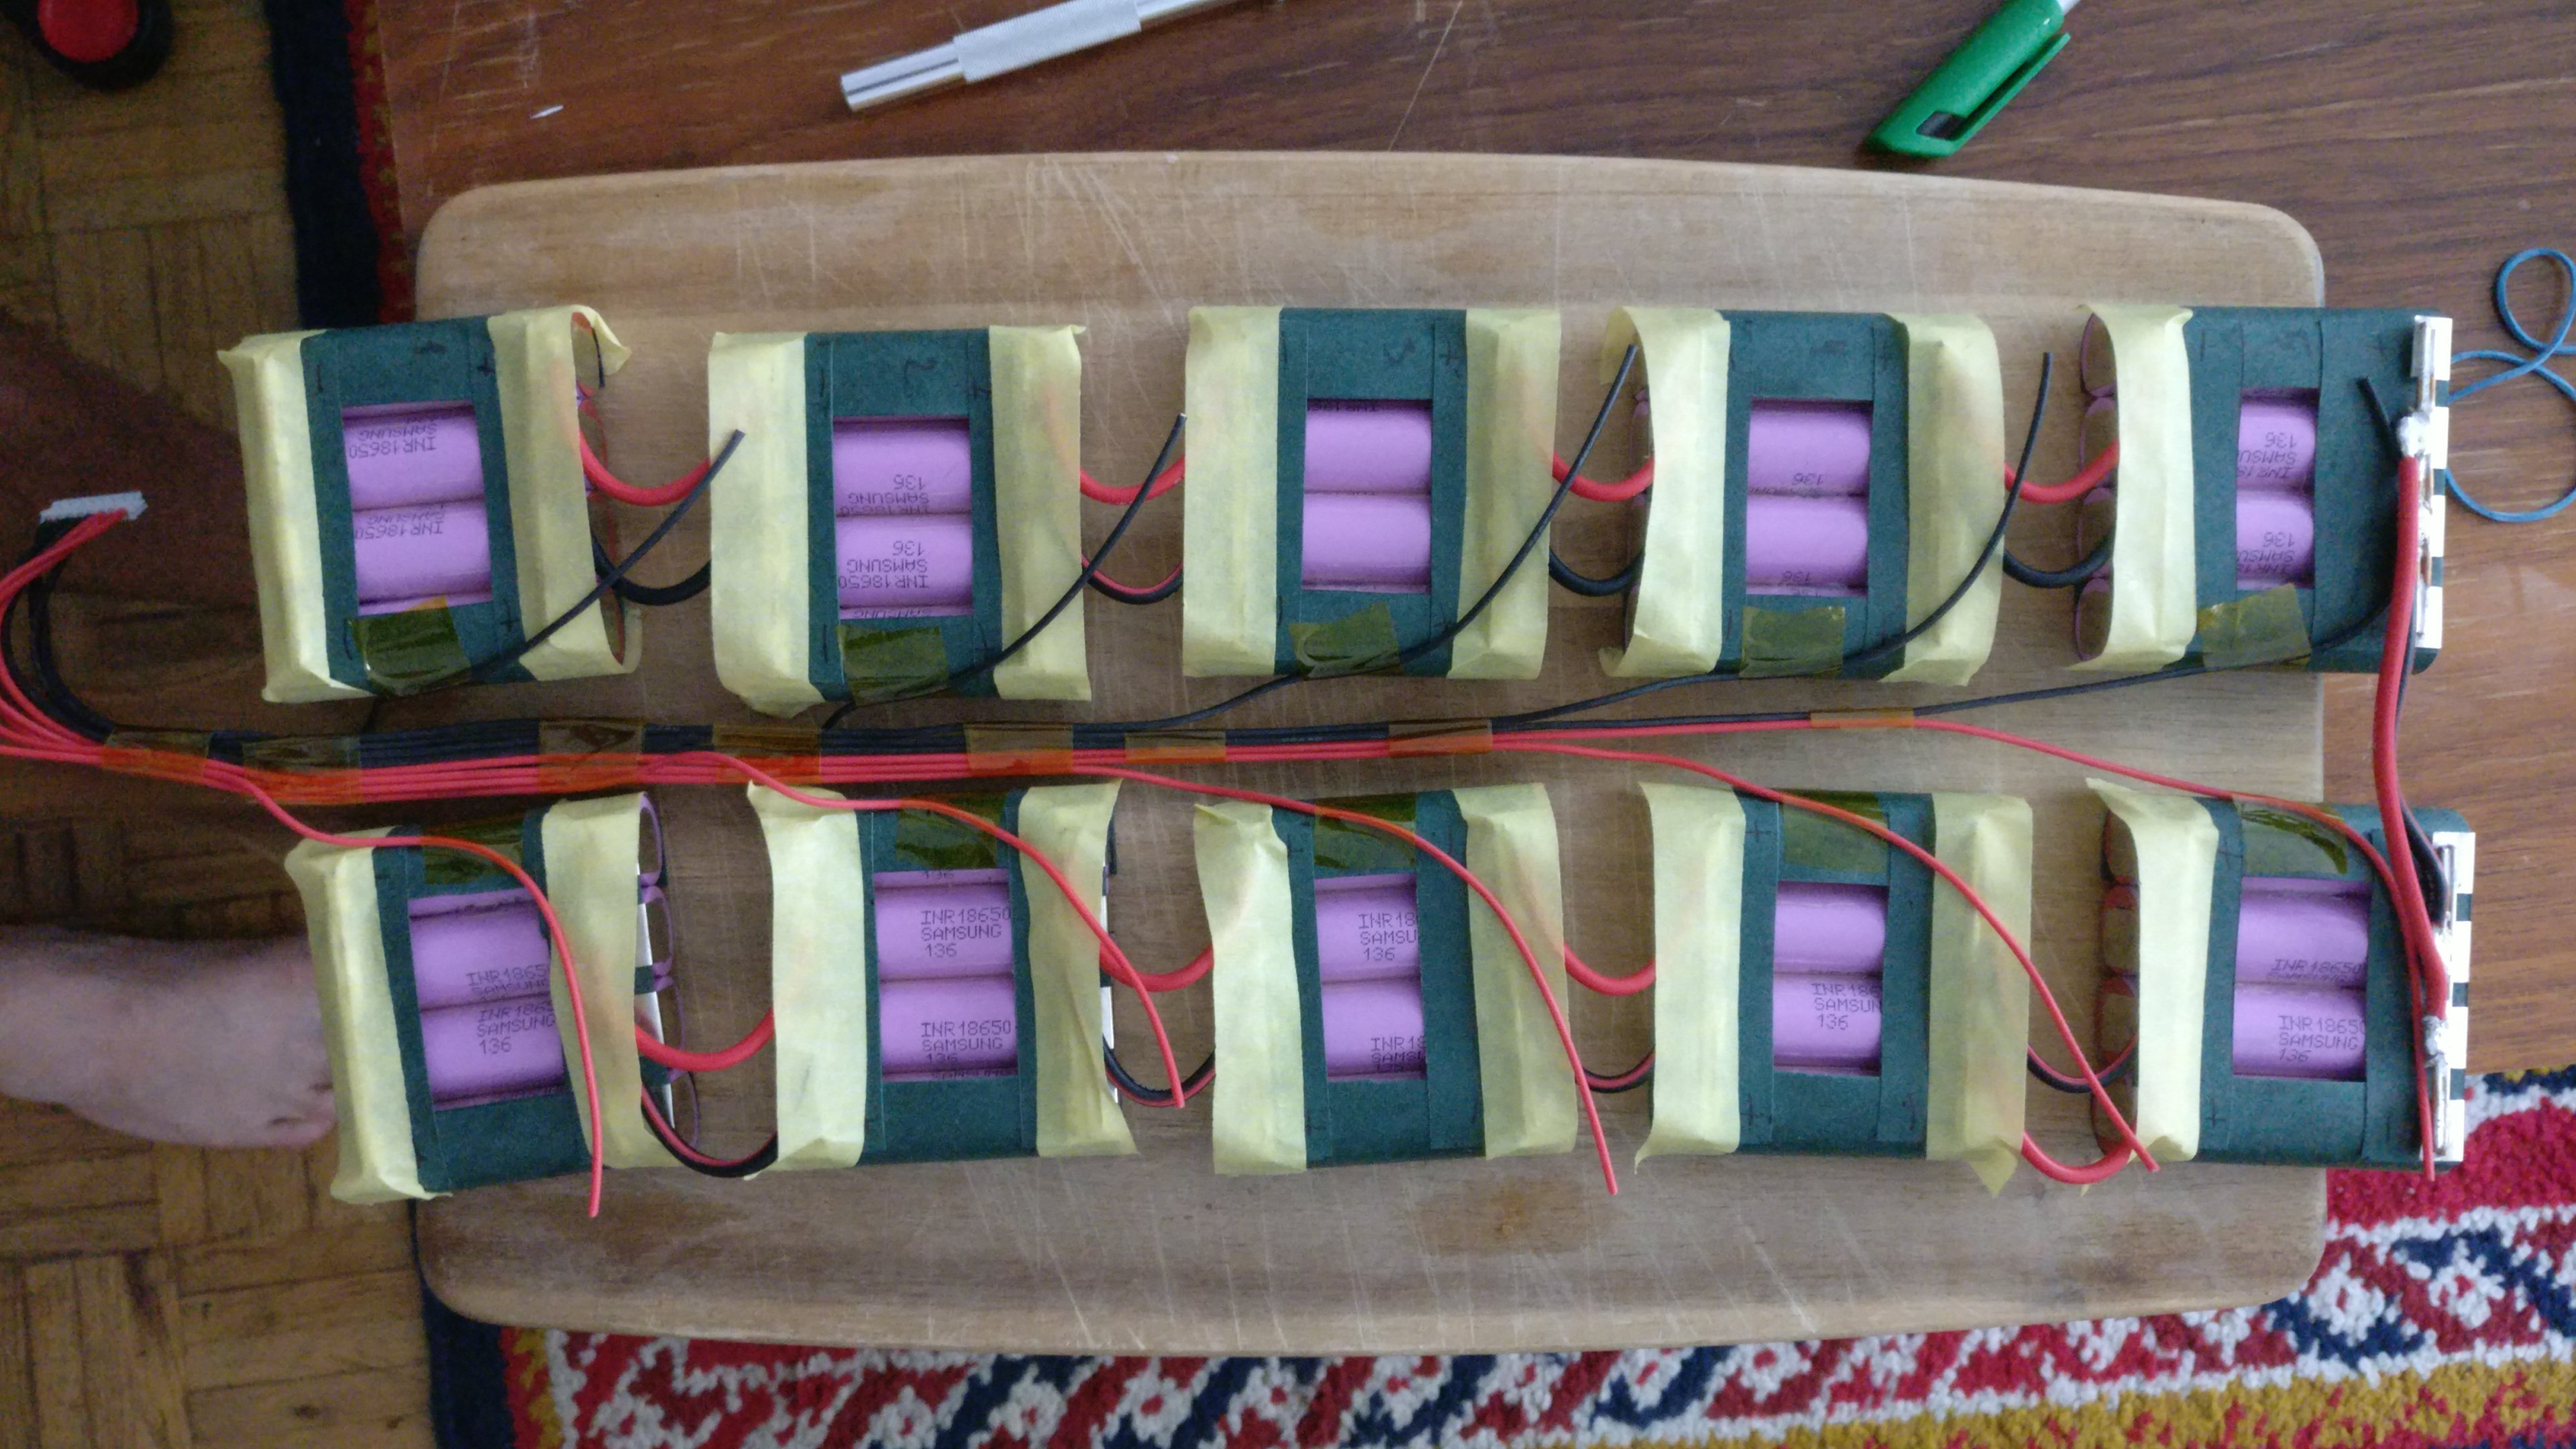
\includegraphics[width=.9\textwidth]{Footage/Pictures/Battery pack.jpg}
				\caption[Der verbaute Lithium-Ionen Zellverband]{Der verbaute Lithium-Ionen Zellverband. Zu erkennen sind die 10 Sub-Zellen bestehend aus jeweils vier Einzelzellen.}\label{fig:battery pack}
			\end{figure}\par
			%
			Das Drehmoment soll durch Elektromotoren erzeugt werden, die von zwei \textit{Elektronischen Speed Controllern} (ESC)\nomenclature[A]{ESC}{Elektronischer Speed Controller} des Typs \textsc{FSESC 4.12}\footnote{Die wiederum industriell gefertigte 1:1 Nachbauten des populären \textsc{VESC} von Benjamin~Vedder sind.} angesteuert werden.
			ESC sind elektronische Komponenten vornehmlich zur elektronischen Kommutation von bürstenlosen Gleichstrommotoren (\textit{Brushless Direct Current}, BLDC).\nomenclature[A]{BLDC}{Brushless Direct Current}
			\begin{figure}[h]
				\centering
				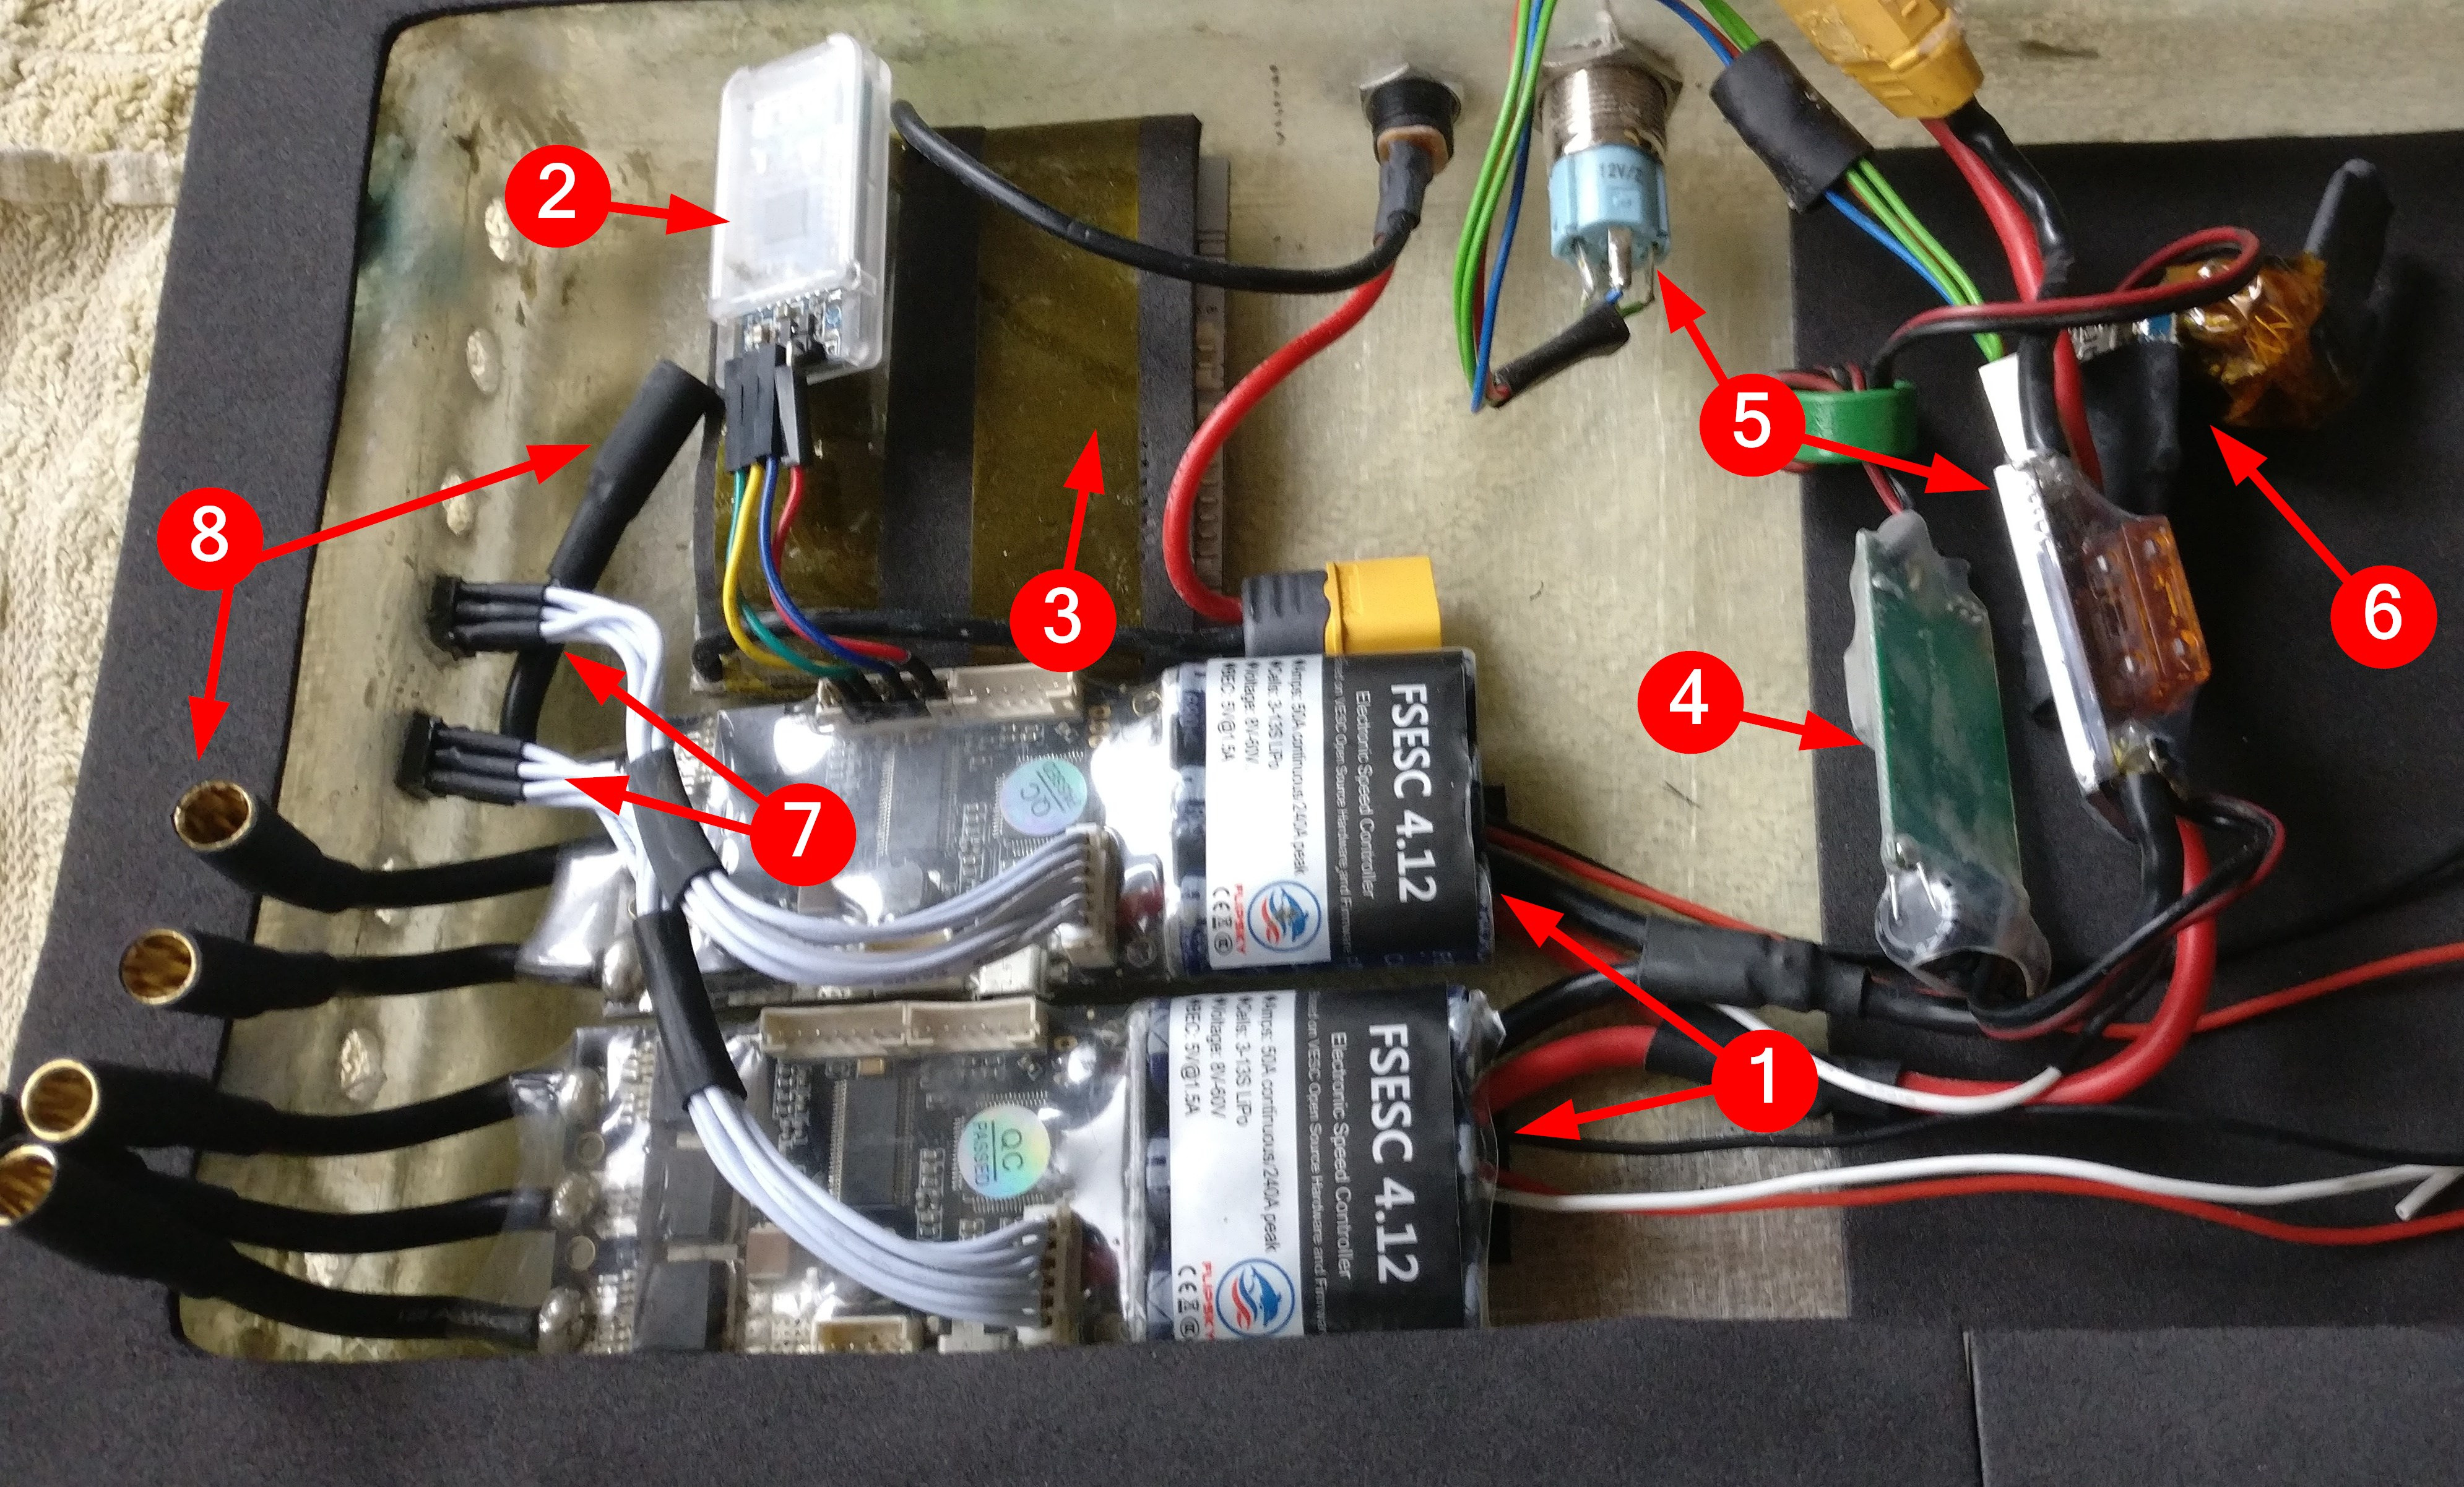
\includegraphics[width=.9\textwidth]{Footage/Pictures/Electronics.jpg}
				\caption[Eingesetzte ESC]{Unten im Bild die beiden eingesetzten ESC vom Typ \textsc{FSESC 4.12}. Weiterhin im Bild zu sehen oben links ein HC-06 Bluetooth Modul, darunter das Batteriemanagementsystem. Auf der rechten Seite im Bild von links nach rechts: Spannungsregler, elektronischer Schalter und der Funkempfänger für die Steuersignale.}\label{fig:electronics}
			\end{figure}
			Als solche schränken sie die Auswahl der Motortypen zwar nicht exklusiv auf BLDCs ein -- Gleichstrommotoren mit Schleifkontakt sind auch denkbar -- allerdings bieten sie in Kombination mit BLDCs einen deutlich höheren Funktionsumfang.
			Darüber hinaus sind BLDC gegenüber Gleichstrommotoren mit Schleifkontakten effizienter, bieten eine höhere Leistungsdichte und sind bauartbedingt unempfindlich gegenüber Nässe\footnote{Je nach Art der Lagerung. Dies betrifft jedoch ausschließlich die mechanischen Komponenten der Motoren.}.
			%
		\subsection{Einsatzumgebung und -bedingungen}
			%
			Das Gewicht des Fahrers wird inklusive Kleidung und transportiertem Gepäck mit \qty{90}{\kilo\gram} angenommen.
			Hinzu zu addieren sind \(\sim \qty{5}{\kilo\gram}\) durch Deck, Batterie und Elektronik und pessimistisch geschätzte weitere \qty{5}{\kilo\gram} durch die beiden Trucks zusammen mit dem Antriebssystem.
			So ergibt sich ein geschätztes, vom Antriebssystem zu beschleunigendes Gesamtgewicht von \(\sim \qty{100}{\kilo\gram}\)\par
			Weiter soll die fertige Maschine auf in urbanen Gebieten üblichen Untergründen betrieben werden können.
			Es wird also mit leichten bis moderaten Steigungen und Asphalt in Form des Bodenbelages gerechnet.\par\medskip
			%
			Die Maschine soll vorrangig als Sportgerät für milde bis sonnige Wetterlagen gedacht werden.
			Extrembedingungen wie Starkregen, Schnee oder Eisglätte finden hier also keine weitere Beachtung.

	\section{Designziele}
		Mit in den obigen Kapiteln genannten Einschränkungen können einige Soll-Forderungen formuliert werden.
		So muss das System\ldots
		\begin{itemize}
			\item \ldots in der Lage sein mindestens das angenommene Gesamtgewicht von \qty{100}{\kilo\gram} moderate Steigungen hinauf befördern zu können.
			Als Designrichtlinie wird hier eine Steigung von \qty{5}{\percent} festgelegt.
			\item \ldots auf ebenem Asphalt auf mindestens \qty{25}{\kilo\metre\per\hour} beschleunigen können.
			In Kombination mit obiger Forderung wird hier auf das Festlegen eines Zeitintervalls, innerhalb dessen die Endgeschwindigkeit erreicht werden soll, verzichtet.
			\item \ldots einfach zu Warten sein.
		\end{itemize}
		Neben den harten Zielen ist wünschenswert, dass das System...
		\begin{itemize}
			\item \ldots möglichst aus selbst herstellbaren Komponenten besteht.
			\item \ldots kostengünstig ist.
			Als Richtwert soll hier \dEUR{300} angelegt werden.
			\item \ldots die von der Batterie zur Verfügung gestellte Leistung von \SI{425}{\watthour} bezogen auf die erreichbare Reichweite möglichst effizient nutzt.
		\end{itemize}